\begin{frame}[c]
    \frametitle{液晶可调谐光谱滤波器:可见光和红外操作}
    \begin{columns}
        \begin{column}{.6\textwidth}
            \begin{itemize}
                \item Gunning, W.;  Pasko, J.; Tracy, J., A \textcolor{purple}{Liquid Crystal} \textcolor{red}{Tunable} Spectral Filter: \textcolor{pink}{Visible And Infrared} Operation. SPIE: 1981; Vol. 0268.
                \item \textcolor{blue}{重要性:}较小范围内的电压调节即可实现较大范围的工作波长。
                \item \textcolor{blue}{瓶颈:}液晶的光学参数与温度有很强的相关性,因此需要研究与热效应有关的问题。
                \item \textcolor{blue}{创新点:}之前的器件在调节通带光谱时所需要的电压非常大,液晶的使用克服了这一限制。
                \item \textcolor{blue}{意义:}有望设计出新的设备,尤其是多个谐振腔的滤波器。
                \item \footnotesize{所使用的材料:\textrm{4-Cyano,-4'-$\eta$-pentylbiphenyl}(4-羟基,-4'-$\eta$-戊基联苯)}
            \end{itemize}
        \end{column}
        \begin{column}{.4\textwidth}
            \begin{figure}[!htb] %H为当前位置,!htb为忽略美学标准,htbp为浮动图形
                \centering %图片居中
                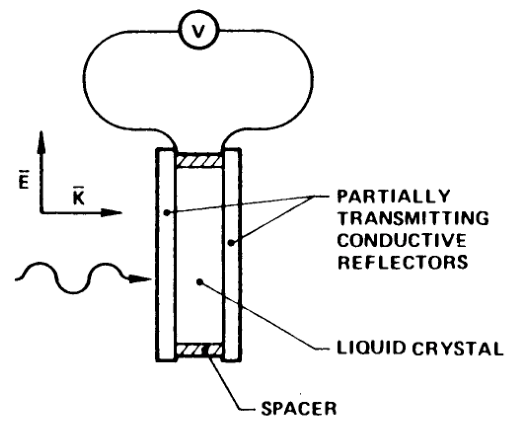
\includegraphics[width=1.\textwidth]{figures/A Liquid Crystal Tunable Spectral Filter Visible And Infrared Operation_1.png} %插入图片,[]中设置图片大小,{}中是图片文件名
                \caption{仪器结构示意图} %最终文档中希望显示的图片标题
            \end{figure}
        \end{column}
    \end{columns}
\end{frame}

\begin{frame}[c]
    \frametitle{液晶可调谐光谱滤波器:可见光和红外操作}
    此仪器是上一篇文章仪器的改进,变化在于谐振腔所使用的介质材料不同。
    \begin{itemize}
        \item 施加不同大小的电压,液晶分子(极化)取向的变化不同。
        \item 有效折射率:$\frac{1}{n(\theta)^2}=\frac{1}{n_\mathrm{o}^2}\cos^2\theta+\frac{1}{n_\mathrm{e}^2}\sin^2\theta$
        \item 典型值:$n_{\mathrm{e}}-n_{\mathrm{o}}=0.2$
    \end{itemize}

    \begin{columns}
        \begin{column}{.5\textwidth}
            \begin{figure}[!htb] %H为当前位置,!htb为忽略美学标准,htbp为浮动图形
                \centering %图片居中
                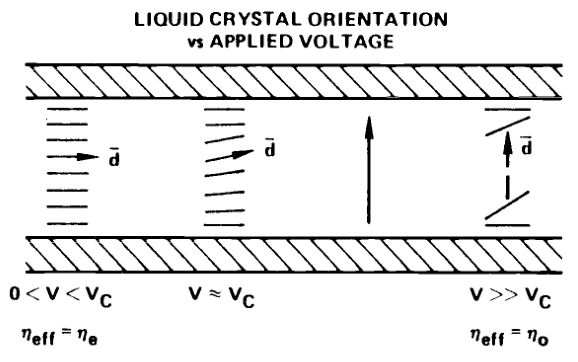
\includegraphics[width=1.\textwidth]{figures/A Liquid Crystal Tunable Spectral Filter Visible And Infrared Operation_2.png} %插入图片,[]中设置图片大小,{}中是图片文件名
                \caption{原理示意图} %最终文档中希望显示的图片标题
            \end{figure}
        \end{column}
        \begin{column}{.5\textwidth}
            \begin{figure}[!htb] %H为当前位置,!htb为忽略美学标准,htbp为浮动图形
                \centering %图片居中
                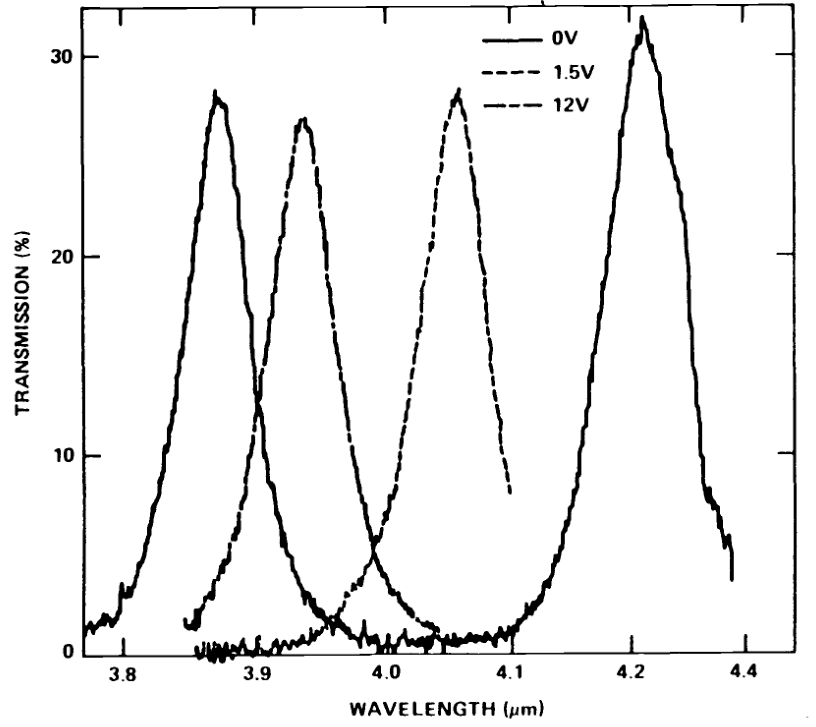
\includegraphics[width=1.\textwidth]{figures/A Liquid Crystal Tunable Spectral Filter Visible And Infrared Operation_3.png} %插入图片,[]中设置图片大小,{}中是图片文件名
                \caption{测试结果} %最终文档中希望显示的图片标题
            \end{figure}
        \end{column}
    \end{columns}
    \begin{itemize}
        \item可以看到,对于上一篇文章来说,现在的仪器用小得多的电压变化实现了大得多的通带波长调节。
    \end{itemize}
\end{frame}